\section{实验协议与审计轨迹}\label{sec:protocol}
\paragraph{同步面板。}每道题由5个Agent进行3轮同步处理。第$t$轮只能观察策略允许的第$t-1$轮报告，同轮Agent彼此不可见。确认性实验使用独立信息条件；受控实验分别暴露新增证据、无证据多数立场、带复制压力的完整报告或立场相反证据。

图~\ref{fig:runtime}给出实现顺序：控制器先承诺，追随者声明行动，执行器运行对应路径，结算后才生成后续历史。失败进入可审计重试或回滚分支。
\begin{figure}[t]\centering
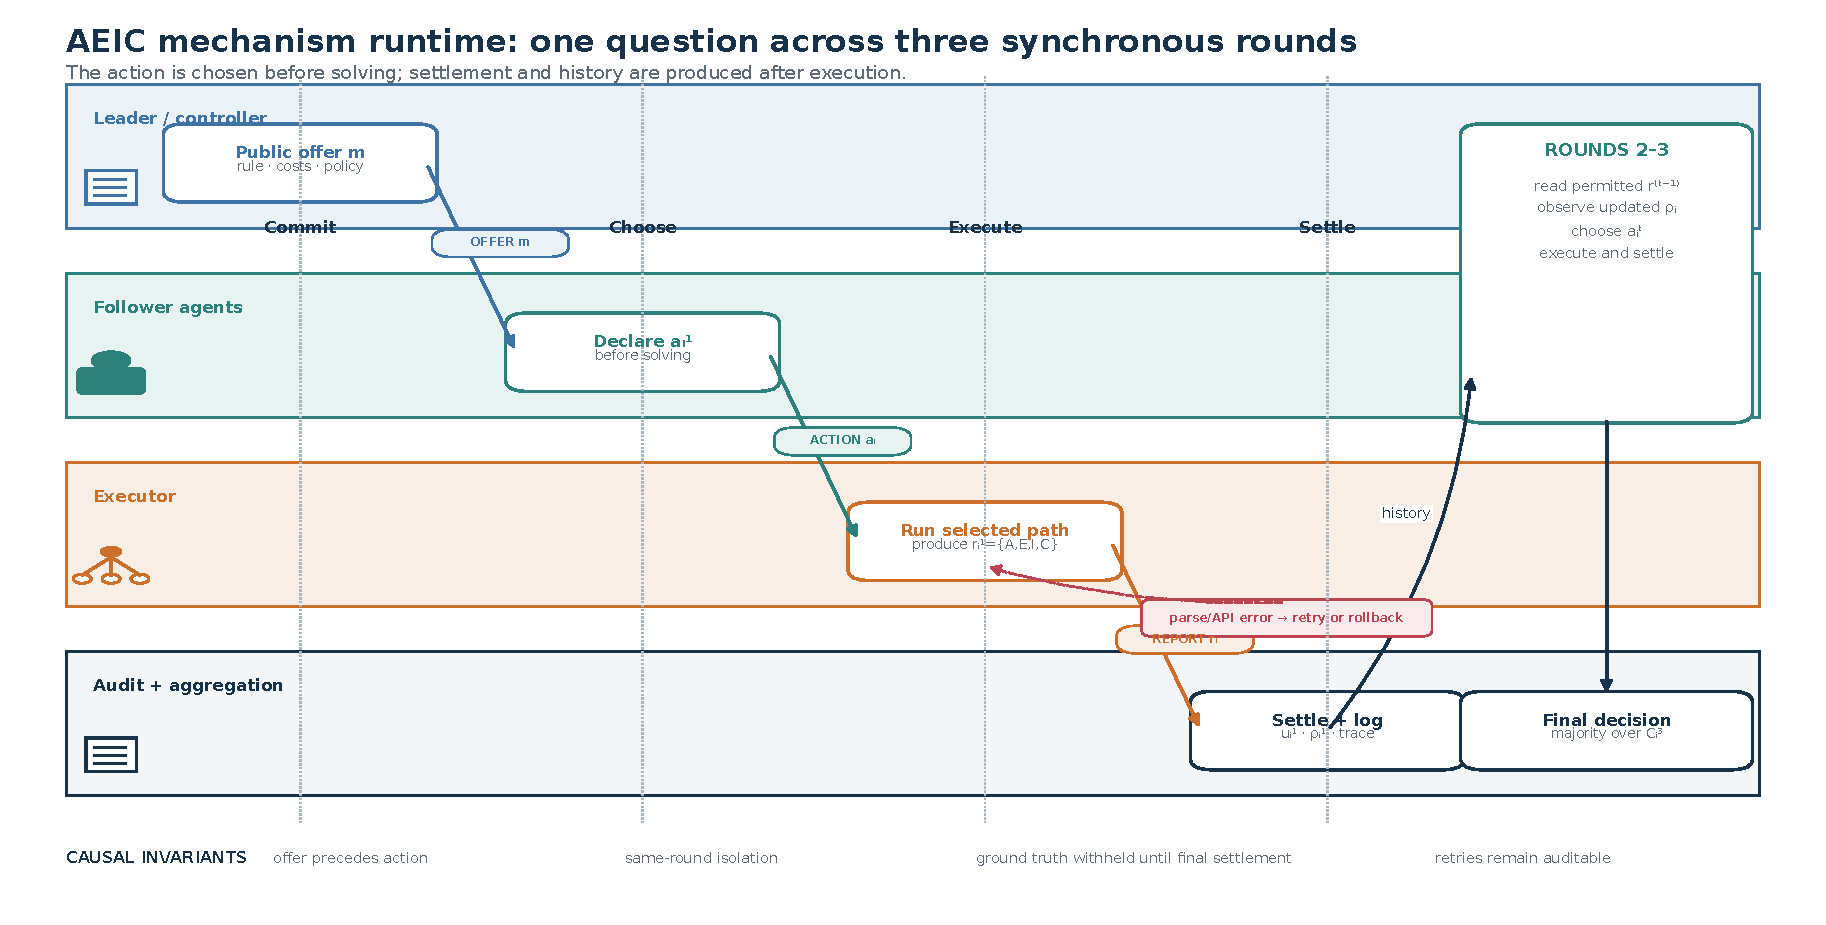
\includegraphics[width=\textwidth]{../figures/fig2_runtime_sequence.pdf}
\caption{单题运行时序。四条泳道区分承诺、选择、强制执行和结算。}\label{fig:runtime}\end{figure}

\paragraph{先选择后执行。}Agent先接收合同、信誉、允许信息和问题并返回单一行动；第二次调用执行行动，\textsc{Verify}增加审计与修订调用。仅解析失败时允许格式修复，且不得改变原结论或添加事实。

\paragraph{配对与聚合。}同一道题的机制共享问题级Seed。最终决策取第三轮$C$字段多数票。高资源行动预先定义为\textsc{AEIC}或\textsc{Verify}。二元结果使用精确McNemar检验，连续结果使用配对秩检验，并在注册比较族内Holm校正。

\paragraph{冻结溯源。}版本化Schema要求记录合同、行动、报告、可见同伴、奖励、成本、信誉、原始响应、Trace、延迟和Token。八组实验共5,850条问题级记录，均通过矩阵、路由和Schema校验，以SHA-256冻结并从标准JSONL独立复算。
